\documentclass[12pt,a4paper]{article} 
\usepackage{graphicx}
\usepackage[portuguese]{babel}
%\usepackage[applemac]{inputenc}
\usepackage[T1]{fontenc}
\usepackage{fullpage}

\usepackage{verbatimbox}
\usepackage{indentfirst} % primeiro par·grado indendado
\usepackage{listings}	 % para colocar cÛdigo fonte

\title{ContinuaÁ„o da segunda avaliaÁ„o de linguagens e compiladores} 
\author{Felipe Giunte Yoshida N$^{\circ}$ USP 4978231\\Mariana Ramos Franco N$^{\circ}$ USP 5179364} 
%\date {29 de Outubro de 2009}

\begin{document} 

\begin{figure}[!t]
\centering 

\includegraphics[width=15.5cm]{logo.pdf}
\end{figure}

\maketitle 

\paragraph{Construa o sistema de programaÁ„o para a linguagem LazyComb que ter· um compilador para a linguagem C, um ambiente de execuÁ„o que contar· com bibliotecas da linguagem. N„o h· E/S na linguagem, mas cada resultado deve ser mostrado na forma de combinadores.}

% LEXICO
\section{LÈxico}
Para implementar o analisador lÈxico utilizamos a mesma estrutura criada para o Compilador FM, sendo necess·rio apenas modificar o arquivo \textbf{automato.xml} com a nova descriÁ„o do autÙmato mostrada a seguir:

\lstset{language=XML, basicstyle=\footnotesize}
\begin{lstlisting}
<gramatica>
	<estado>
		<id>0</id>
		<final>false</final>
		<tipo>0</tipo>
		<transicao>
			<entradas>ISK()</entradas>
			<proximo>1</proximo>
		</transicao>
	</estado>
	<estado>
		<id>1</id>
		<final>true</final>
		<tipo>1</tipo>
	</estado>
</gramatica>
\end{lstlisting} 

Como pode-se notar, o lÈxico aceita somente as entradas 'I','S', 'K', '(' e ')'. Assim, nosso compilador n„o trata entradas no formato Unlambda, Iota ou Jot.

% SINTATICO
\section{Sint·tico}
Assim como o lÈxico, tambÈm utilizamos a estrutura montada para o compilador FM para implementar o sint·tico.
Foi necess·rio alterar a o arquivo \textbf{gram·tica.txt} de entrada para o meta-analisador com a gram·tica da linguagem Lazy-K na notaÁ„o de Wirth:

\lstset{language=C, basicstyle=\footnotesize}
\begin{lstlisting}
Program = { Expr } .

Expr = "I" | "K" | "S" | "(" { Expr } ")" .
\end{lstlisting}

Desta maneira obtemos o autÙmato de pilha estruturado da linguagem como mostrado nas figuras \ref{fig:program} e \ref{fig:expr}.

\begin{figure}[ht!]
	\begin{center}
		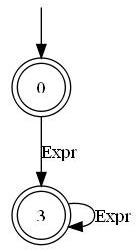
\includegraphics[scale=0.60]{program.jpg}
		\caption{Subm·quina 'Program'}
		\label{fig:program}
	\end{center}
\end{figure}

\begin{figure}[ht!]
	\begin{center}
		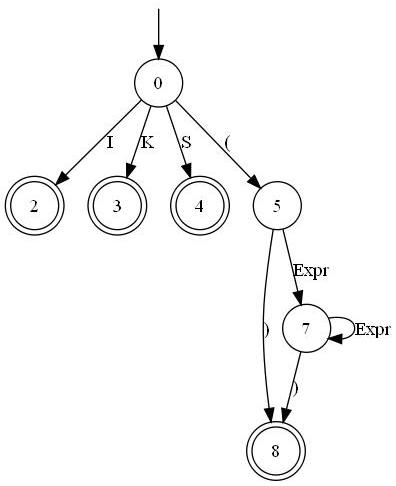
\includegraphics[scale=0.60]{expr.jpg}
		\caption{Subm·quina 'Expr'}
		\label{fig:expr}
	\end{center}
\end{figure}

TambÈm alteramos a classe \textbf{Sintatico.java} para que esta passasse a chamar corretamente os autÙmatos 'Program' ou 'Expr' conforme os tokens recebidos e o valor no topo da pilha estado-subm·quina.


% SEMANTICO
\section{Sem‚ntico}
Para fazer a an·lise sem‚ntica e gerar o cÛdigo em C, respons·vel por reduzir a cadeia contida no arquivo \textbf{arquivofonte.lazy}, criamos uma nova classe \textbf{Semantico.java} que È chamada pelo sint·tico ‡ cada transiÁ„o nos autÙmatos 'Program' ou 'Expr'.

Basicamente o que o sem‚ntico faz È escrever no arquivo final as seguintes chamadas de funÁ„o conforme o valor do token consumido:

\lstset{language=Java, basicstyle=\footnotesize}
\begin{lstlisting}
			if(token.getValor().equals("S")){
				main = "entra('S');";
				main = "tenta_reduzir();";
				
			}else if(token.getValor().equals("K")){
				main = "entra('K');";
				main = "tenta_reduzir();";
				
			}else if(token.getValor().equals("I")){
				main = "entra('I');";
				main = "tenta_reduzir();";
				
			}else if(token.getValor().equals("(")){
				main = "novo_escopo();";
				
				
			}else if(token.getValor().equals(")")){
				main = "fecha_escopo();";
				main = "tenta_reduzir();";
\end{lstlisting} 


% SEMANTICO
\section{Ambiente de ExecuÁ„o}

O ambiente de execuÁ„o consiste em 5 funÁıes, descritas abaixo:

\paragraph{novo\_escopo} Abre um novo escopo, que ocorre quando se encontra uma abertura de parÍnteses.

\paragraph{entra} Insere um novo caracter no atual escopo

\paragraph{tenta\_reduzir} Tenta fazer uma das reduÁıes ($I x \rightarrow x$, $K x y \rightarrow x$ ou $S x y z \rightarrow ( x z ) ( x y )$) no escopo atual

\paragraph{fecha\_escopo} Fecha escopo atual e copia resultado para o escopo anterior

\paragraph{imprime} Imprime cadeia do escopo atual

\section{Testes}


Para a entrada \verb|I(KKI)(IIKSI)|, chegamos a um código em C, que não será colocado no relatório por seu tamanho.

Ao se executar este código em um compilador C, chegamos ao seguinte resultado:

\begin{verbatim}
Caractere adicionado I
I
Novo escopo nivel 1

Caractere adicionado K
K
Caractere adicionado K
KK
Caractere adicionado I
KKI
Reduziu K
K
Escopo nivel 1 fechado
IK
Reduziu I
K
Novo escopo nivel 1

Caractere adicionado I
I
Caractere adicionado I
II
Reduziu I
I
Caractere adicionado K
IK
Reduziu I
K
Caractere adicionado S
KS
Caractere adicionado I
KSI
Reduziu K
S
Escopo nivel 1 fechado
KS
KS

\end{verbatim}

\end{document} 